\documentclass[a4paper]{article}

%% Language and font encodings
\usepackage[english]{babel}
\usepackage[utf8x]{inputenc}
\usepackage[T1]{fontenc}

%% Sets page size and margins
\usepackage[a4paper,top=3cm,bottom=2cm,left=3cm,right=3cm,marginparwidth=1.75cm]{geometry}

%% Useful packages
\usepackage{amsmath}
\usepackage{amsthm}
\usepackage{filecontents}
\usepackage{graphicx}
\usepackage{fancyhdr}
\usepackage{geometry}
\usepackage{parskip}
\usepackage{amsfonts}
\usepackage{pdfpages}
\usepackage{tabularx}
\usepackage{bm}
\usepackage{mathtools}
\usepackage[normalem]{ulem}
\usepackage{verbatim}
\usepackage{tikz}
\usepackage{pgfplots}
\pgfplotsset{compat=1.14}
\usepgfplotslibrary{patchplots}

\usetikzlibrary{calc,matrix,plothandlers,plotmarks,shapes}


\begin{document}

\begin{center}
    \Huge\bfseries{Gradient Descent: The Beginning of the Robot Apocalypse}
    \small\text{It's not going to be funny when it's \textit{you} being localized by the killbots}
\end{center}
\vspace{1in}

\section*{What is it and why do I care?}

So say we have the following graph:\\\\
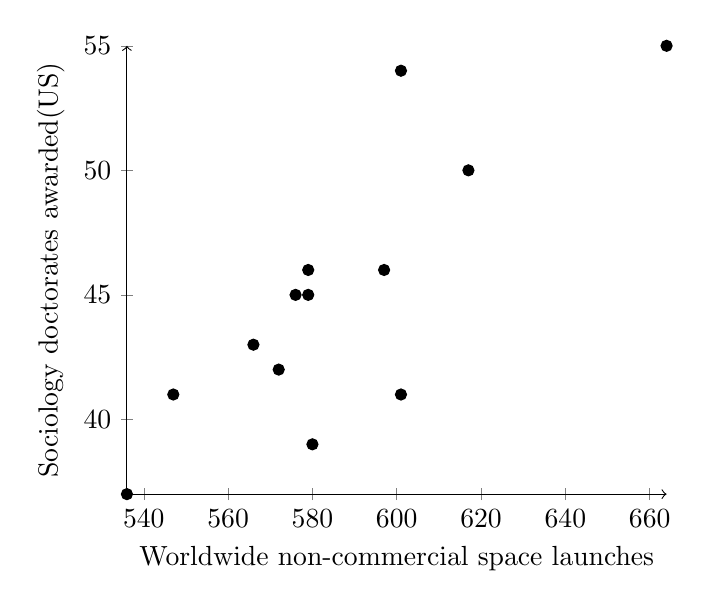
\begin{tikzpicture}
    \begin{axis}[axis lines=middle, axis line style={->}, ylabel near ticks, xlabel near ticks, xlabel={Worldwide non-commercial space launches}, ylabel={Sociology doctorates awarded(US)}]
        % \addplot[black,samples=100,domain=0:1] {120*(1-x)^(1/3)-1};
        \addplot[domain=500:700, only marks, error bars/.cd, error bar style={color=mapped color}]
            table[x=x,y=y,x error=xerr,y error=yerr]{
                x       xerr    y        yerr       class
                601     0.00000 54       0.00000    0
                579     0.00000 46       0.00000    0
                572     0.00000 42       0.00000    0
                617     0.00000 50       0.00000    0
                566     0.00000 43       0.00000    0
                547     0.00000 41       0.00000    0
                597     0.00000 46       0.00000    0
                580     0.00000 39       0.00000    0
                536     0.00000 37       0.00000    0
                579     0.00000 45       0.00000    0
                576     0.00000 45       0.00000    0
                601     0.00000 41       0.00000    0
                664     0.00000 55       0.00000    0
            };

    \end{axis}
\end{tikzpicture}

Let's find the line of best fit between the number of worldwide non-commercial space launches and sociology doctorates awarded in the US\@. How hard can it be?

Ok so let's just think of some values for a simple linear fit, $y = mx+b$.\\\\
Maybe... \bm{$m=0.001,\, b=30$}?$ $\\

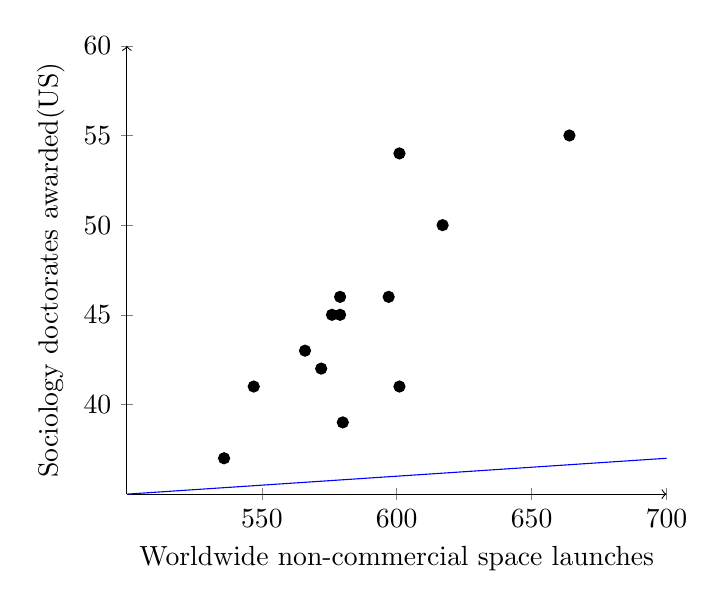
\begin{tikzpicture}
    \begin{axis}[axis lines=middle, axis line style={->}, ylabel near ticks, xlabel near ticks, xlabel={Worldwide non-commercial space launches}, ylabel={Sociology doctorates awarded(US)}, xmin=500,xmax=700,ymin=35,ymax=60,restrict y to domain=0:5600]
        \addplot[only marks, error bars/.cd, error bar style={color=mapped color}]
            table[x=x,y=y] {
                x   y 
                601 54 
                579 46 
                572 42 
                617 50 
                566 43 
                547 41 
                597 46 
                580 39 
                536 37 
                579 45 
                576 45 
                601 41 
                664 55 
            };
        \addplot[color=blue, domain=450:700] {x/100 + 30};
    \end{axis}
\end{tikzpicture}
\\\\
Ok, no, that sucked. Let's try \bm{$m=0.001,\, b=0$}?\\
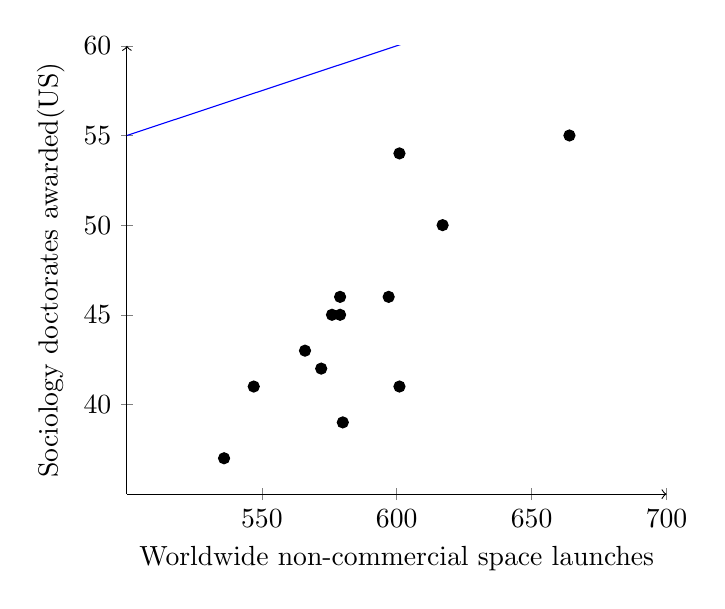
\begin{tikzpicture}
    \begin{axis}[axis lines=middle, axis line style={->}, ylabel near ticks, xlabel near ticks, xlabel={Worldwide non-commercial space launches}, ylabel={Sociology doctorates awarded(US)}, xmin=500,xmax=700,ymin=35,ymax=60,restrict y to domain=0:5600]
        \addplot[only marks, bars/.cd]
            table[x=x,y=y]{
                x   y 
                601 54 
                579 46 
                572 42 
                617 50 
                566 43 
                547 41 
                597 46 
                580 39 
                536 37 
                579 45 
                576 45 
                601 41 
                664 55 
            };
        \addplot[color=blue, domain=450:700] {x*0.05 + 30};
    \end{axis}
\end{tikzpicture}

Wow, humans sure suck at things. So how should we fit the line? Calculators probably don't just randomly guess... right?
\\\\If you guessed "right," you're correct. I think.
\\\\\\
It's time for...
\vspace{-22pt}
\section*{Gradient Descent!}

So, what do we want to minimize? Well, error.\\

But how do we define error?

Here's an idea. Let's define it in a completely arbitrary way: mean square error.
What this means is that $error_{total} = \dfrac{\sum{error^2}}{numofpoints}$, or that the total error is defined as the average of the squares of each of the individual errors, or distance from points to the line.

\DeclarePairedDelimiter\abs{\lvert}{\rvert}%
\DeclarePairedDelimiter\norm{\lVert}{\rVert}%

Thanks to our friends Gibbs and Heaviside, we can find the shortest distance between a point and a line using vector projection, and generalize it to define the distance from any point $(x_0, y_0)$ to a line $ax + by + c$ as\\\\
\vspace{-22pt}
\begin{center}
    $error = \dfrac{\abs{a\cdot x_0 + b\cdot y_0 + c}}{\sqrt{a^2 + b^2}}$
\end{center}

Of course, $b$ is effectively redundant since $a$ and $c$ is all you need to fully define a 2D line, so we can just set $b$ to 1.
So, with that being said, let's transform our above equation, knowing this, into slope-intercept form.

\begin{center}
    $error = \dfrac{\abs{-a\cdot x_0 + y_0 + -b}}{\sqrt{(-a)^2 + 1}}$
\end{center}

I know this is true because I graphed it in desmos and it looked like it worked.


Anyways, our graph of worldwide non-commercial space launches vs. sociology doctorates awared in the US has a total of 13 data points. Meaning this is going to kind of suck.\\

Anyways, here's the entire equation defining the error function of our line given the paramters $m$ and $b$. You're just going to have to take my word on the data because tables are hard apparently.\\

$\dfrac{\abs{-m\cdot 601 + 54 + -b}}{\sqrt{(-m)^2 + 1}} + \dfrac{\abs{-m\cdot 579 + 46 + -b}}{\sqrt{(-m)^2 + 1}} + \dfrac{\abs{-m\cdot 572 + 42 + -b}}{\sqrt{(-m)^2 + 1}} + \dfrac{\abs{-m\cdot 617 + 50 + -b}}{\sqrt{(-m)^2 + 1}} + \dfrac{\abs{-m\cdot 566 + 43 + -b}}{\sqrt{(-m)^2 + 1}} + \dfrac{\abs{-m\cdot 547 + 41 + -b}}{\sqrt{(-m)^2 + 1}} + \dfrac{\abs{-m\cdot 597 + 46 + -b}}{\sqrt{(-m)^2 + 1}} + \dfrac{\abs{-m\cdot 580 + 39 + -b}}{\sqrt{(-m)^2 + 1}} + \dfrac{\abs{-m\cdot 536 + 37 + -b}}{\sqrt{(-m)^2 + 1}} + \dfrac{\abs{-m\cdot 579 + 45 + -b}}{\sqrt{(-m)^2 + 1}} + \dfrac{\abs{-m\cdot 576 + 45 + -b}}{\sqrt{(-m)^2 + 1}} + \dfrac{\abs{-m\cdot 601 + 41 + -b}}{\sqrt{(-m)^2 + 1}} + \dfrac{\abs{-m\cdot 664 + 55 + -b}}{\sqrt{(-m)^2 + 1}}$  \\

Luckly, assuming m is positive, this all compresses down to:\\\\
$error = \dfrac{\abs{584 - 7615x - 13y}}{\sqrt{m^2+1}}$ \\

This is cool. We now have an equation giving us an $error$ $function$ of our parameters to the linear equation ($m$ and $b$).

So what does it look like if we graph this?

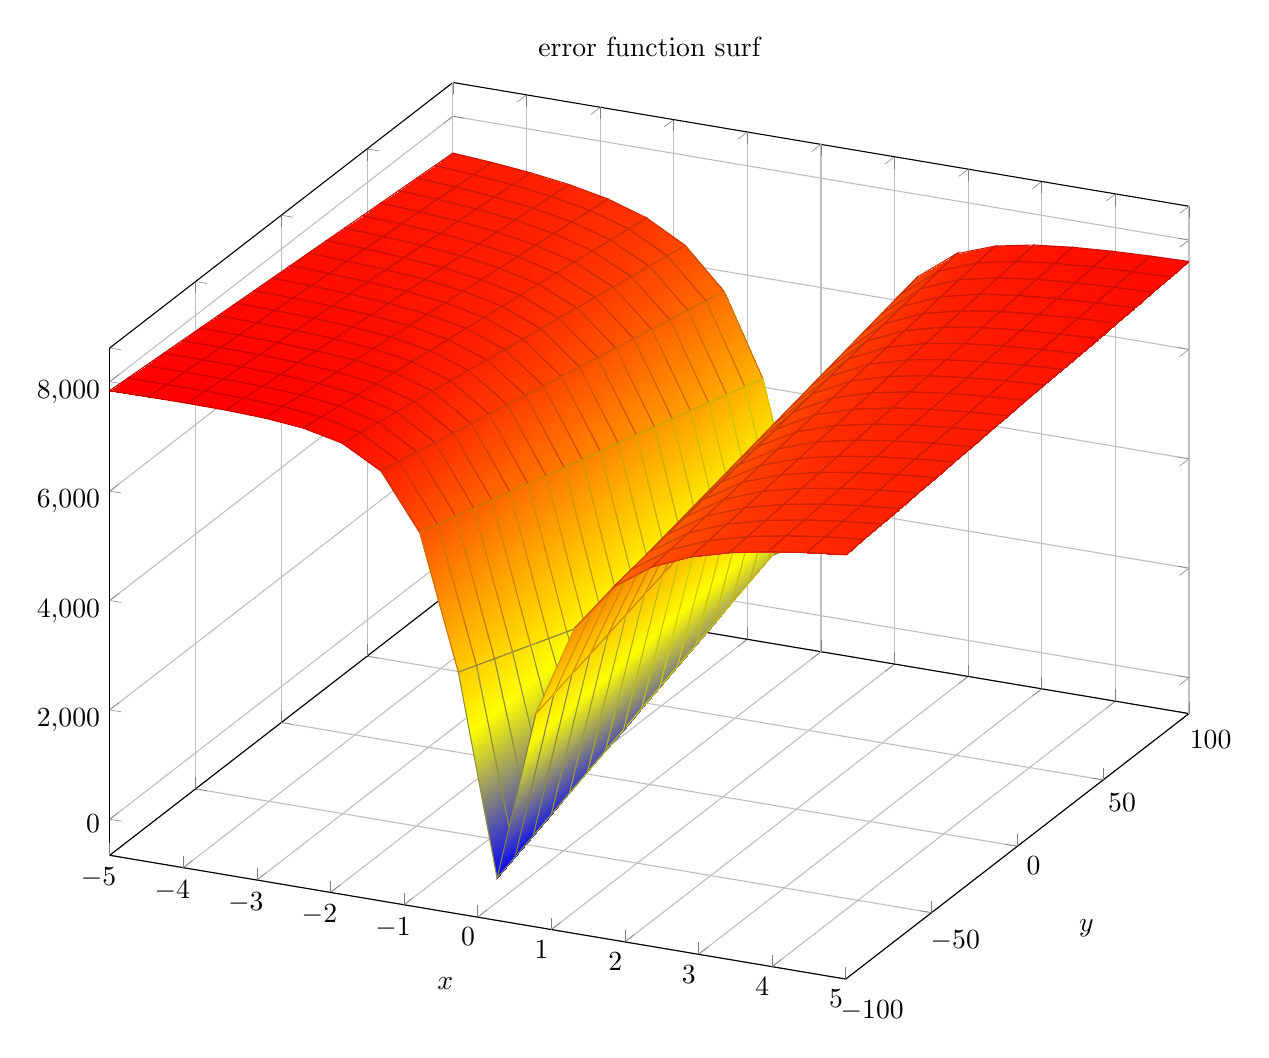
\begin{tikzpicture}
    \begin{axis}[grid=both,scale=2.0, xmin=-5, xmax=5,ymin=-100,ymax=100,xlabel=$x$,ylabel=$y$, title=error function surf]
        % \addplot3[surf,shader=faceted interp] {|584 - 7615x - 13y|/sqrt(m^2 + 1)};
        \addplot3[surf,samples=20,shader=faceted interp, domain=-5:5, domain y=-100:100] {abs(584 - 7615*x - 13*y)/sqrt(x*x + 1)};
    \end{axis}
\end{tikzpicture}

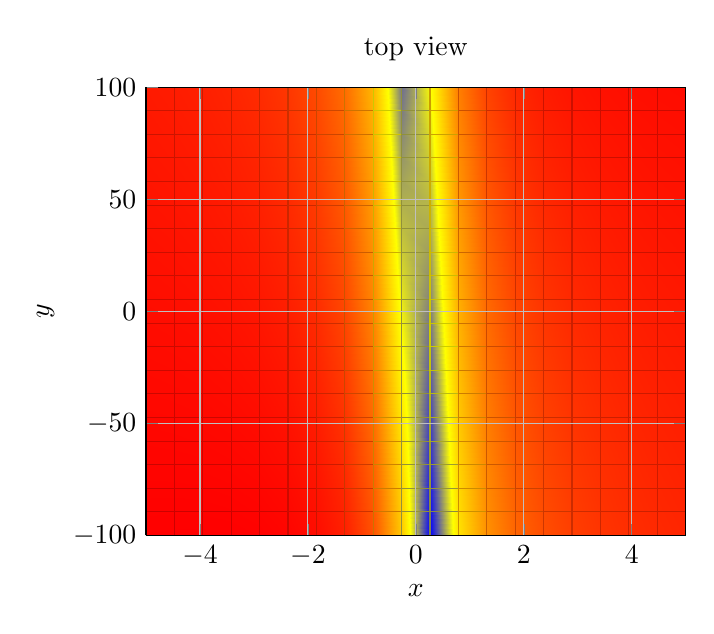
\begin{tikzpicture}
    \begin{axis}[grid=both,scale=1.0, xmin=-5, xmax=5,ymin=-100,ymax=100,xlabel=$x$,ylabel=$y$, view={0}{90}, title=top view]
        % \addplot3[surf,shader=faceted interp] {|584 - 7615x - 13y|/sqrt(m^2 + 1)};
        \addplot3[surf,samples=20, shader=faceted interp, domain=-5:5, domain y=-100:100] {abs(584 - 7615*x - 13*y)/sqrt(x*x + 1)};
    \end{axis}
\end{tikzpicture}
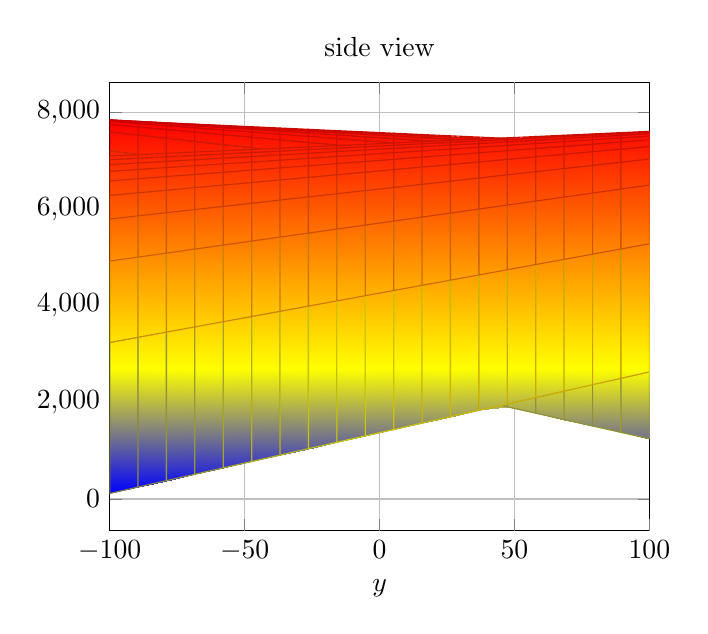
\begin{tikzpicture}
    \begin{axis}[grid=both,scale=1.0, xmin=-5, xmax=5,ymin=-100,ymax=100,xlabel=$x$,ylabel=$y$, view={90}{0}, title=side view]
        % \addplot3[surf,shader=faceted interp] {|584 - 7615x - 13y|/sqrt(m^2 + 1)};
        \addplot3[surf,samples=20, shader=faceted interp, domain=-5:5, domain y=-100:100] {abs(584 - 7615*x - 13*y)/sqrt(x*x + 1)};
    \end{axis}
\end{tikzpicture}

Wow thats cool, it's a really bad paper plane. Yay now we have the error function, and this paper is over. Cool see ya thanks.


\section*{but wait there's more}

ok but so how do we get the line of best fit from this?

\renewcommand{\ULthickness}{2.0pt}%
Using \sout{\textbf{\textit{SCIENCE!}}} \textbf{\textit{MATHEMATICS!}}
\renewcommand{\ULthickness}{.4pt}% Resetting to ulem default

So let's pick a point $(x, y)$ on the domain of $x\in[-5, 5]$ and $y\in[-100,100]$.\\

How about $(3, 30)$? Inputting that into our error function gives $\approx7162.87$. That's a lot (I think) but we can minimize that in a second.

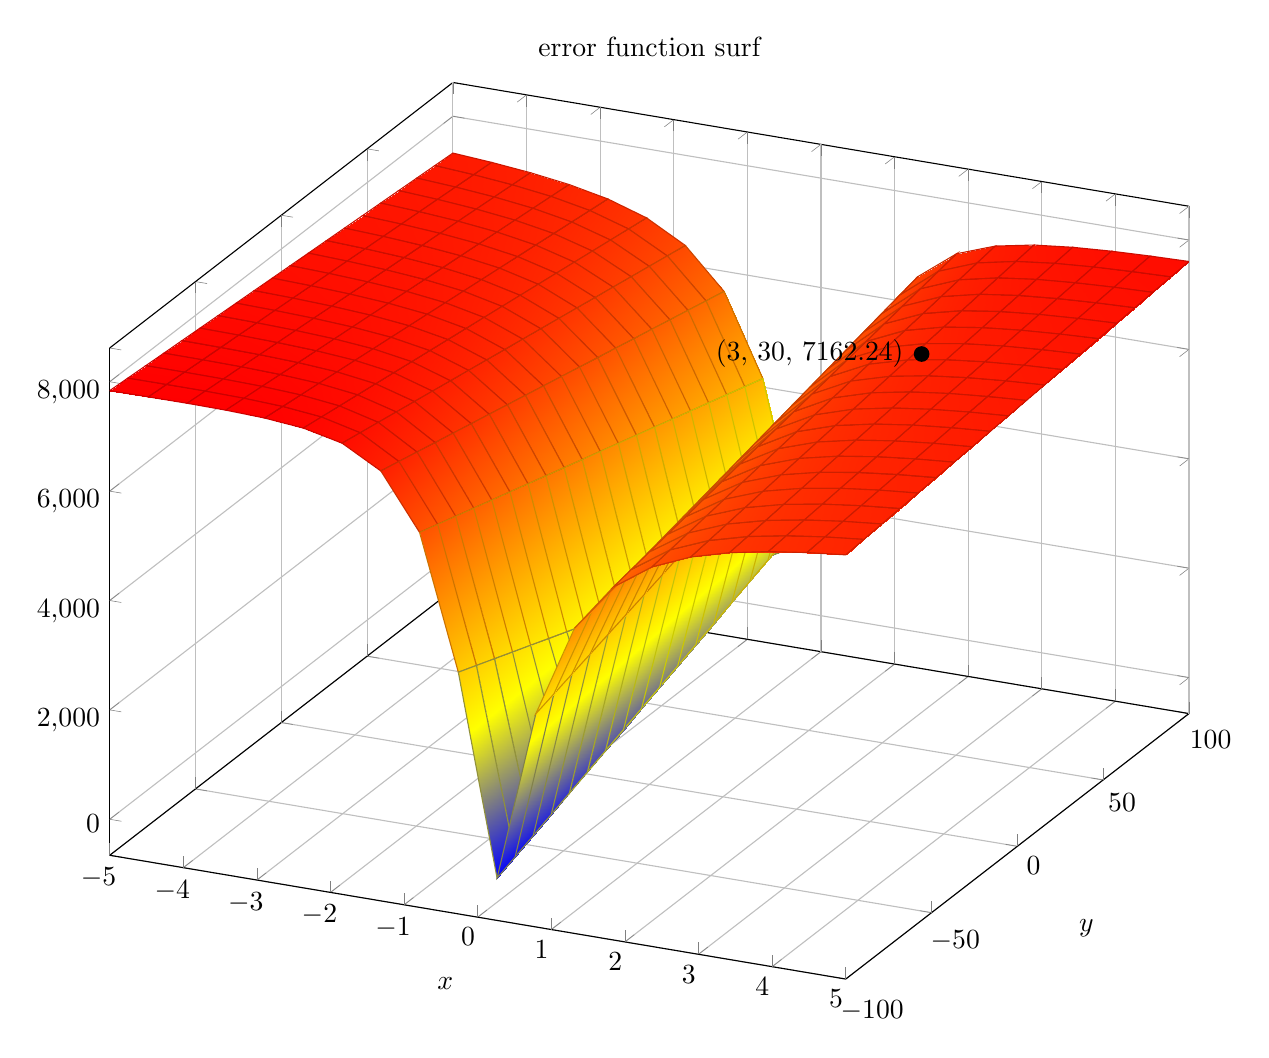
\begin{tikzpicture}
    \begin{axis}[grid=both,scale=2.0, xmin=-5, xmax=5,ymin=-100,ymax=100,xlabel=$x$,ylabel=$y$, title=error function surf]
        % \addplot3[surf,shader=faceted interp] {|584 - 7615x - 13y|/sqrt(m^2 + 1)};
        \addplot3[surf,samples=20,shader=faceted interp, domain=-5:5, domain y=-100:100] {abs(584 - 7615*x - 13*y)/sqrt(x*x + 1)};
        \addplot3[mark=*] coordinates {(3, 30, 7162.24)};
        \node[label={180:{(3, 30, 7162.24)}},circle,fill,inner sep=2pt] at (axis cs:3,30,7162.24) {};

    \end{axis}
\end{tikzpicture}


So if you recall, the equation for total error is $\dfrac{\abs{584 - 7615x - 13y}}{\sqrt{x^2+1}}$. So how do we minimize the error based on that? Well if you're in some lame Calc AB course the answer will be find all the minima. Unfortunately, you can't feasibly do that in more advanced equations like differential equations and big neural networks. However, derivatives can still help.\\

What happens if we take the 2D derivative AKA gradient vector? That's $\nabla f(x_0, y_0)$, or in more specific terms,
$\begin{bmatrix}
\dfrac{\partial x}{\partial z}, \dfrac{\partial y}{\partial z}
\end{bmatrix}$.
Cool. So, entering the total error equation into totally not wolframalpha, we determine the overall vector gradient function to be

\begin{center}
    $
    \nabla f(x, y) = 
    \begin{bmatrix}
        \dfrac
        {7615(x^2 + 1)(7615x + 13y - 584) - x\abs{-7615x - 13y + 584}^2}
        {(x^2 + 1)^(3/2) \abs{-7615x - 13y + 584}},
        \dfrac
        {13(7615x + 13y + 584)}
        {\sqrt{x^2 + 1}\abs{-7615x - 13y + 584}}
    \end{bmatrix}
    $
\end{center}


That's a handful, but thankfully we have computers.

So at $(3, 30)$, that'll be $\begin{bmatrix}-260.40, -4.11\end{bmatrix}$. That means that if we want to $descend$ along the gradient, we just "step" $away$ from the gradient vector (because the gradient vector is the direction of maximum gradient increase).\\

Let's try that. Keep in mind the current error is $\approx 7162.24$ at $(3, 30)$ with a gradient of $\begin{bmatrix}-259.40, -4.11\end{bmatrix}$.\\
A step size of $1\cdot10^{-3}$ means that we'll update the $x$-coordinate from $3$ to $3 + (-1) \cdot -259.40 \cdot 1\cdot10^{-3}$, and the $y$-coordinate from $30$ to $30 + (-1) \cdot -4.11 \cdot 1\cdot10^{-3}$. This results in a new point of $\begin{bmatrix}-2.7406, 30.00411\end{bmatrix}$. Now, the new error is $\approx7086.45$.\\


So what if we use the magic power of computers to do this a bunch of times?

\begin{tikzpicture}
    \begin{axis}[grid=both,scale=2.0, xmin=-5, xmax=5,ymin=-100,ymax=100,xlabel=$x$,ylabel=$y$, title=error function surf]
        % \addplot3[surf,shader=faceted interp] {|584 - 7615x - 13y|/sqrt(m^2 + 1)};
        \addplot3[surf,samples=20,shader=faceted interp, domain=-5:5, domain y=-100:100] {abs(584 - 7615*x - 13*y)/sqrt(x*x + 1)};
        \addplot3[mark=*] coordinates {(3, 30, 7162.24)};
        \node[label={180:{(3, 30, 7162.24)}},circle,fill,inner sep=2pt] at (axis cs:3,30,7162.24) {};
        % \addplot3[black, smooth] table[x=a, y=b, z=c, col sep=comma, mark=none, smooth] {file.csv};
        \addplot3[black, smooth] table[x=a, y=b, z=c, col sep=comma, mark=none, smooth] {file2.csv};
    \end{axis}
\end{tikzpicture}

\begin{tikzpicture}
    \begin{axis}[grid=both,scale=1.0, xmin=-5, xmax=5,ymin=-100,ymax=100,xlabel=$x$,ylabel=$y$, title=error function surf, view={0}{90}]
        % \addplot3[surf,shader=faceted interp] {|584 - 7615x - 13y|/sqrt(m^2 + 1)};
        \addplot3[surf,samples=20,shader=faceted interp, domain=-5:5, domain y=-100:100] {abs(584 - 7615*x - 13*y)/sqrt(x*x + 1)};
        \addplot3[mark=*] coordinates {(3, 30, 7162.24)};
        \node[label={180:{(3, 30, 7162.24)}},circle,fill,inner sep=2pt] at (axis cs:3,30,7162.24) {};
        % \addplot3[black, smooth] table[x=a, y=b, z=c, col sep=comma, mark=none, smooth] {file.csv};
        \addplot3[black, smooth] table[x=a, y=b, z=c, col sep=comma, mark=none, smooth] {file2.csv};
    \end{axis}
\end{tikzpicture}

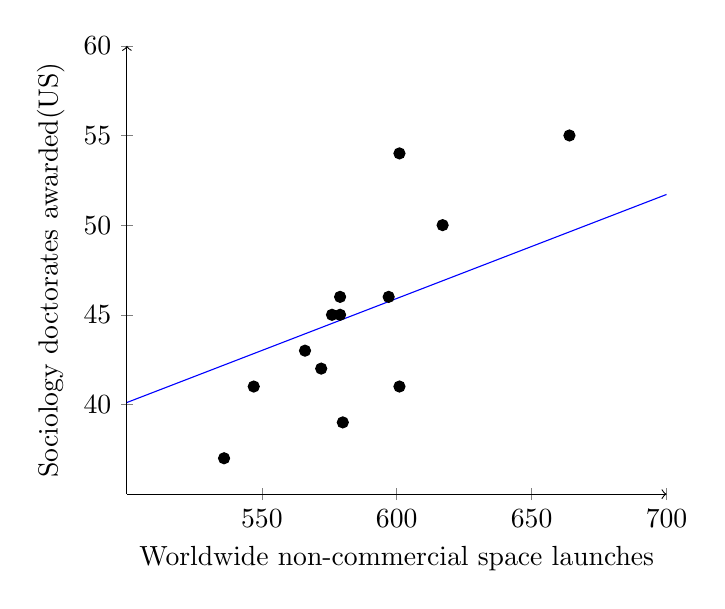
\begin{tikzpicture}
    \begin{axis}[axis lines=middle, axis line style={->}, ylabel near ticks, xlabel near ticks, xlabel={Worldwide non-commercial space launches}, ylabel={Sociology doctorates awarded(US)}, xmin=500,xmax=700,ymin=35,ymax=60,restrict y to domain=0:5600]
        \addplot[only marks, error bars/.cd, error bar style={color=mapped color}]
            table[x=x,y=y] {
                x   y 
                601 54 
                579 46 
                572 42 
                617 50 
                566 43 
                547 41 
                597 46 
                580 39 
                536 37 
                579 45 
                576 45 
                601 41 
                664 55 
            };
        \addplot[color=blue, domain=450:700] {0.05800704203777168*x + 11.10655031880448};
    \end{axis}
\end{tikzpicture}


Et voila, that's gradient descent.\\\\
Now normally you'd use a "real" descent algorithm like Stochastic Gradient Descent or Adadelta, not a cobbled-together python implimentation that I'm pretty sure I defined the loss function wrong for. But yeah, that's a kinda cool probably extremely flawed implementation, and the $\nabla$ symbol looks pretty cool.

\end{document}


